\chapter{Method}
This chapter describes the material used for testing, the method for testing, the environment setup and the test cases that has been conducted. First, a survey for selecting the air quality monitors that will be used in this research are introduced. Then, the technical architecture and setup for each device are explained. The test environment for the devices and the hardware and software are presented to ensure reproducibility. At last, the test cases conducted are derived and presented. 
\section{Air Quality Monitor Survey}
For selection of material, the problem description and research questions have been used as a reference. In order to answer the RQs the air quality monitors needs to be manufactured from different vendors. To find the specific AQMs to use in this research, several online sources are used and compared. As this research is conducted on NTNU Gjøvik in Norway, it is also preferable that the devices are bought and available in Norwegian stores or online pages. The devices chosen should also be popular and easy accessible for any user. It exists many solutions that integrate air quality monitors within other devices, but as this thesis aims to investigate what private information are possible to infer from an air quality monitor, the devices chosen should only have air quality monitoring functionality.  Considering these factors, the following guidelines are made out to select the devices:
\begin{itemize}
    \item The devices are be manufactured from different vendors
    \item The devices communicates over Wi-Fi
    \item The devices are available for any user
    \item The devices only monitors indoor air quality
    \item The devices should preferably be available in Norwegian stores
\end{itemize}
Tibber \cite{Tibber} is a Norwegian power company that specializes in combining smart technology, as with IoT devices, and live app representaion of the power consumption and smart devices \cite{Tibber}.  Tibber has over 400.000 users in Northern Europe Which makes them a natural choice for many when integrating a smart home device to their environment \cite{TibberUsers}. On their webpage it is possible to buy several IoT smart devices for your home. Here they recommend one AQM which communicates over Wi-Fi, Netatmo Healthy Home Coach. Netatmo \cite{Netatmo} is a company that specializes in consumer technology. They have one indoor air quality monitor and which uses four sensors to present the indoor air quality of an environment. These are; humidity, \(CO_2\), noise and temperature. 
\\\\
Elkjøp \cite{Elkjøp} and Komplett \cite{Komplett} are two of Norways biggest electrical stores with a wide range of different smart home devices both in store and online. Its therefore a natural choice when users are looking for any electronic devices including smart devices. When searching for "Air Quality Monitors" on their webpages, Elkjøps shows 4 different vendors and Komplett 8 different vendors. Both vendors lists Netatmo Healthy Home coach, which is already chosen. A part from this both Elkjøp and Komplett also recommends Mill Sense air quality monitor. Mill \cite{Mill} is a Norwegian company that manufactures and sells products for indoor climate and heating, with the goal of developing devices that fits the indoor interior environment. They offer one air quality monitor called Mill Sense which communicates over Wi-Fi. The sensors integrated are \(eCO_2\), humidity, temperature and TVOC.
\\\\
When sorting the devices on client reviews on Komplett, the highest ranking manufacturer of air quality monitors is Nedis \cite{Komplett}. Nedis \cite{Nedis} is an electronic company with the goal of making electronic-related solutions based on the newest technology. They have different solutions for air quality monitors, but the one that communicates over Wi-Fi is called Nedis SmartLife Air Quality Monitor WiFi. This device monitors \(CO_2\), HCHO, humidity, temperature and VOCs and communicates over WiFi. 
\\\\
The research will consists of air quality monitors from the selected three different vendors. The devices only works as air quality monitors and they have different sensors. The chosen devices from the survey are represented underneath in a summarized table. 
\begin{table}[!hbtp]
    \centering
    \begin{adjustbox}{width=1\textwidth}
    \begin{tabular}{| p{3cm} | p{5cm} | p{5cm} | p{3cm} |} 
        \hline
        \textbf{Vendor} & \textbf{Air Quality Monitor} & \textbf{Communication protocol} & \textbf{Sensors} \\
        \hline
        Mill & Sense Smart Climatesensor & WiFi & \(eCO_2\) \newline Humidity \newline Temperature \newline TVOC \\
        \hline
        Nedis & SmartLife Air Quality Monitor & WiFi & \(CO_2\) \newline HCHO \newline Humidity \newline Temperature \newline VOC \\
        \hline
        Netatmo & Smart Air Quality Monitor & WiFi & \(CO_2\) \newline Noise \newline Humidity \newline Temperature \\
        \hline
    \end{tabular}
    \end{adjustbox}
    \caption{Air Quality Monitor Devices}
    \label{tab:AQMSurvey}
\end{table}
\FloatBarrier

\subsection{Mill Sense Air Quality Monitor}
Mill Sense Air Quality Monitor measures the indoor air quality with 4 different sensors: humidity, TVOC, Temperature and \(eCO_2\). \cite{Mill} The monitor communicates to the users mobile phone through WiFi and connects it data to Mills own app called \textit{Mill Norway}. It is possible to use Mill Sense together with other Mill units to change their values based on the sensor data from Mill Sense. 
\\\\
\textit{Figure \ref{fig:MillSenseBoth}} shows Mill Sense and its corresponding application, Mill Norway. 
\begin{figure} [!ht]
    \centering
    \begin{subfigure}{0.3\textwidth}
         \centering
         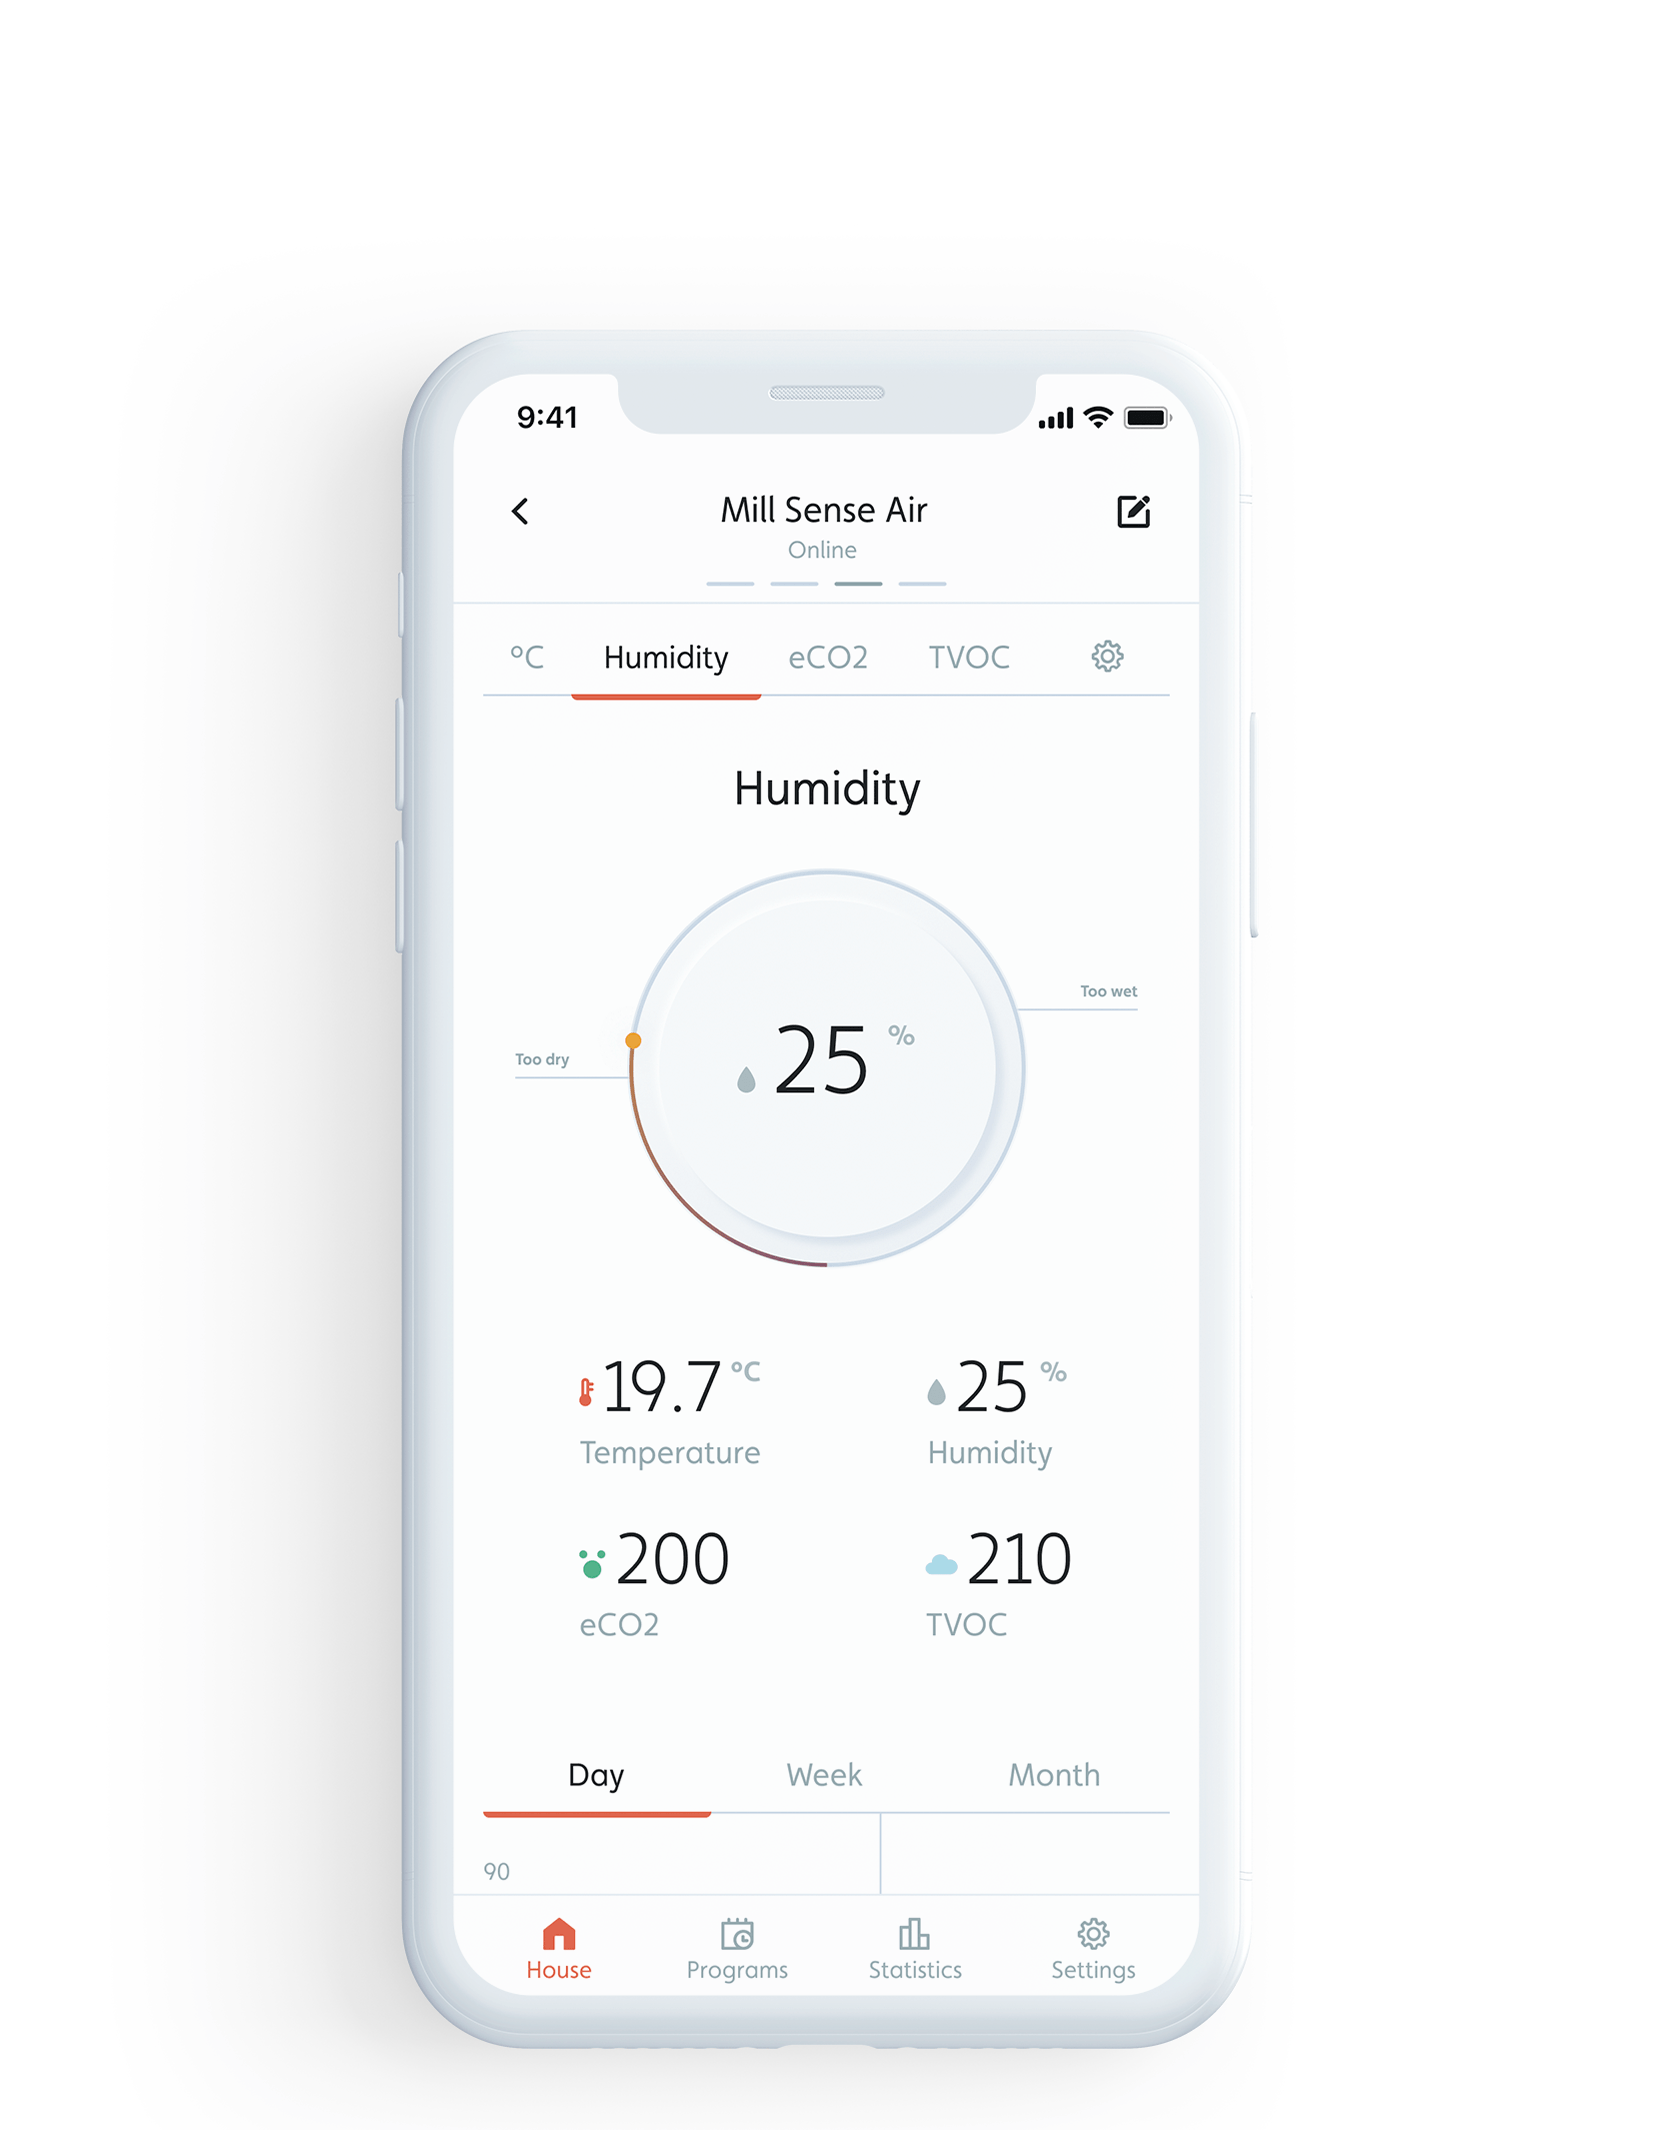
\includegraphics[width=1.5\textwidth]{figures/MillSenseApp.png}
         \caption{Mill Norway \cite{MillSense}}
         \label{fig:MillSenseApp}
     \end{subfigure}
     \hfill
      \begin{subfigure}{0.3\textwidth}
         \centering
         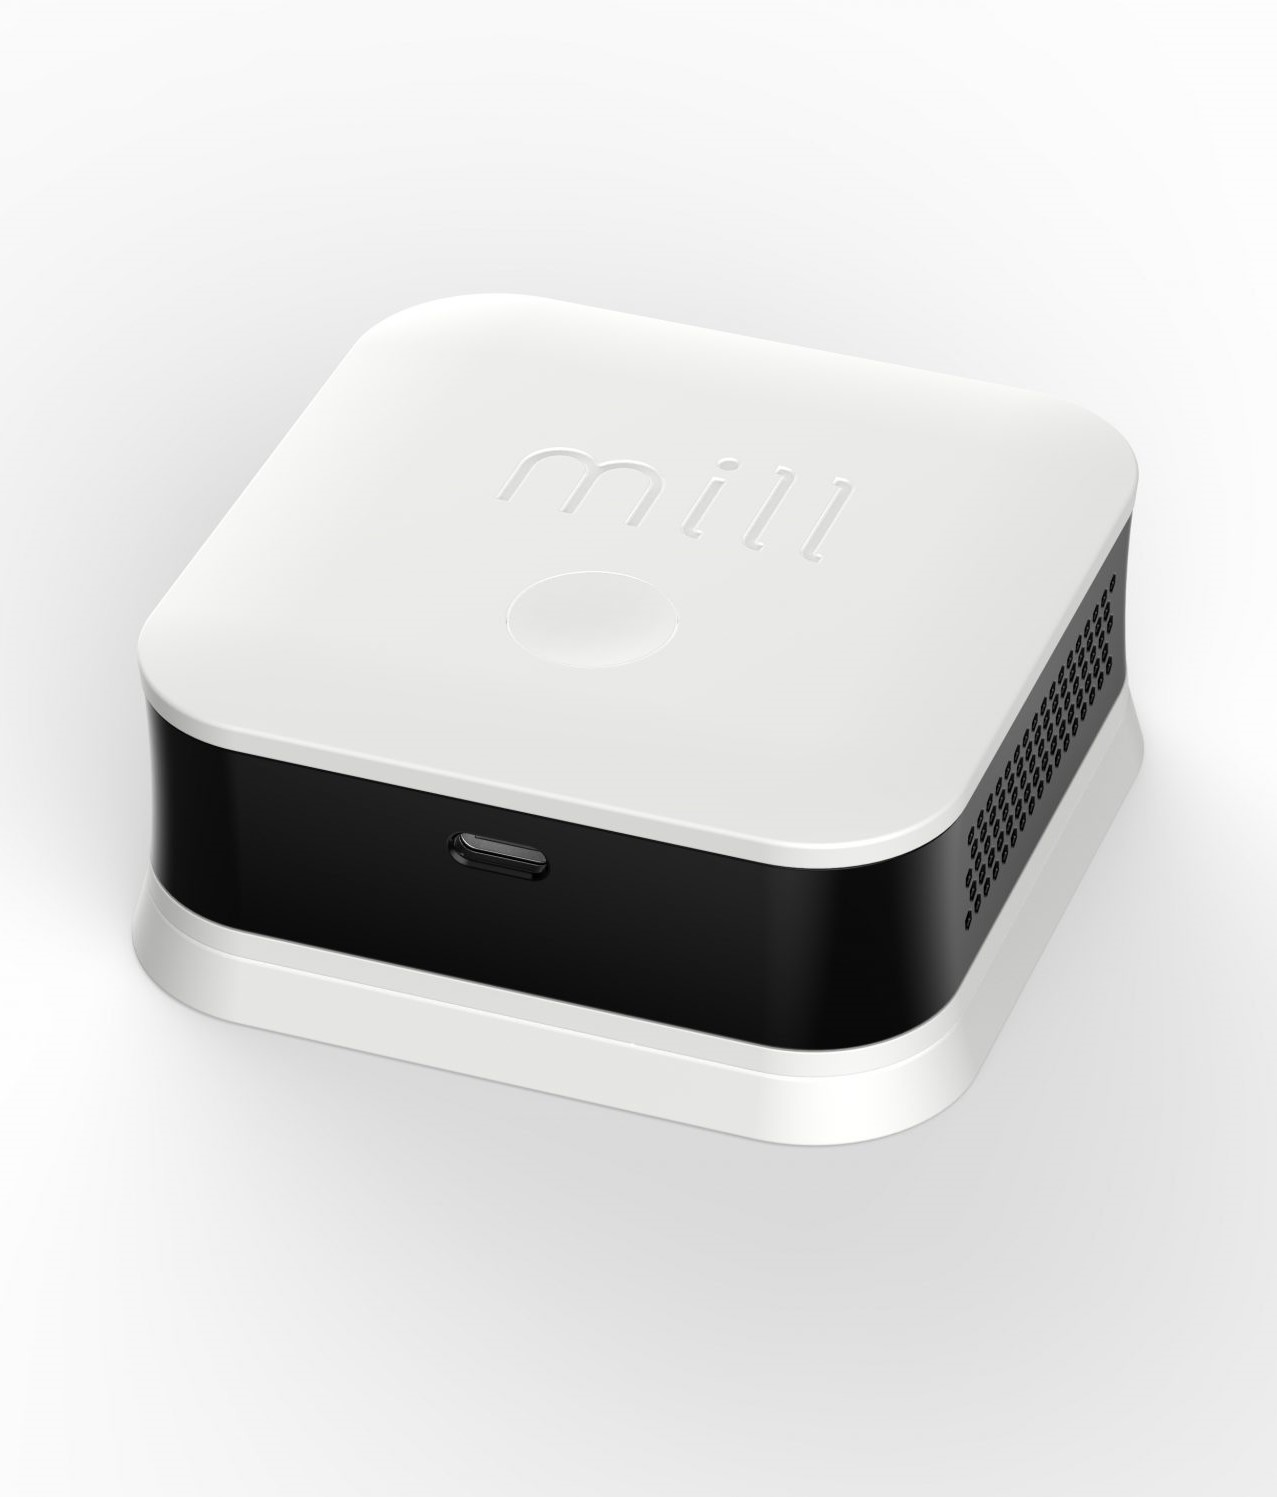
\includegraphics[width=1.5\textwidth]{figures/MillSense.jpg}
         \caption{Mill Sense device \cite{MillSense}}
         \label{fig:MillSenseDev}
     \end{subfigure}
     \hfill
        \caption{Mill Sense}
        \label{fig:MillSenseBoth}
\end{figure}
\\\\
Mill has a privacy policy regarding their collection of user data from all of their devices \cite{MillPrivacy}. The personal data described to be collected are User Profile, Usage, Device, Location and Crash data. User Profile data includes name, address, telephone number, e-mail address, users daily schedule and other information attached to functions of the device. Usage data contains performance and climate conditions in the users house. The Device data will gather information about when to update and mobile user identification information unique for each mobile phone. Location data sends the SSID for the device to the app, even though the app is not in use. Crash data are used to gather information when the device is not working properly \cite{MillPrivacy}. 
\\\\
The AQM does not need power to stay connected and can be placed in any preferred room. The app does not provide notifications to users of threshold levels, but displays the current levels in the app together with graphs that shows variations back in time. Instead of sending notifications to a users phone, the device shows different light responses on the physical unit. These threshold values can be customized. The sensor data collected from the environment is sent to the cloud and back to the users app. It is possible to choose interval for sensor data, from every minute to every hour. When the unit is turned on for the first time and installed in the environment, the device needs at least 5 days to calibrate its sensors. 
\\
\subsection{Nedis SmartLife Air Quality Monitor}
Nedis SmartLife Air Quality monitor have 3 different indoor AQM sensors; humidity, temperature and VOC \cite{NedisDevice}. The monitor communicates over Wi-Fi to the app, \textit{Nedis SmartLife}. As Nedis have several other smart devices, the unit can be integrated in a smart environment together with other devices. 
\\\\
\textit{Figure \ref{fig:NedisBoth}} shows Nedis SmartLife Air Quality Monitor and its corresponding application, Nedis SmartLife. 
\begin{figure} [!ht]
    \centering
    \begin{subfigure}{0.3\textwidth}
         \centering
         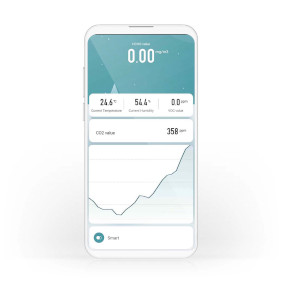
\includegraphics[width=1.5\textwidth]{figures/NedisApp.jpg}
         \caption{Nedis SmartLife App \cite{Nedis}}
         \label{fig:NedisApp}
     \end{subfigure}
     \hfill
      \begin{subfigure}{0.3\textwidth}
         \centering
         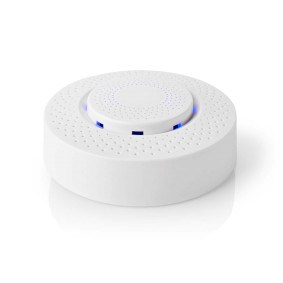
\includegraphics[width=1.5\textwidth]{figures/NedisDevice.jpg}
         \caption{Nedis SmartLife Air Quality Monitor \cite{Nedis}}
         \label{fig:NedisDev}
     \end{subfigure}
     \hfill
        \caption{Nedis SmartLife}
        \label{fig:NedisBoth}
\end{figure}
\\\\
Nedis privacy policy states that they automatically collects device information, usage data, log information and smart device related information, such as device name, id, status, version and upgrade. There will be carried out statistical analysis to imporve the application and devices to the users needs. They also disclose some of the data to third party services to be able to provide some of their services. 
\\\\
The Nedis SmartLife does not have notification default setup, but it can easily be set by the user. Every sensor reading from the device can be set to notify both when levels are too high or too low, meaning that the user can set its own thresholds. The readings on this app shows live data as well as a graphical view of previous readings up to a year before. For setup in an environment, Nedis does not specify any calibration time.  

\subsection{Netatmo Smart Indoor Air Quality Monitor}
The Netatmo Smart Indoor Air Quality Monitor entails 4 different sensors; humidity, \(CO_2\), noise and temperature. It can be integrated with several smart indoor air quality monitor devices placed around in users home. It communicates over WiFi to their own app called \textit{Healthy Home Coach}. The device can be integrated with other smart home devices using HomeKit. 
\\\\
\textit{Figure \ref{fig:Netatmo}} shows Netatmo Healthy Home Coach and its corresponding application, Healthy Home Coach. 
\begin{figure} [!ht]
    \centering
    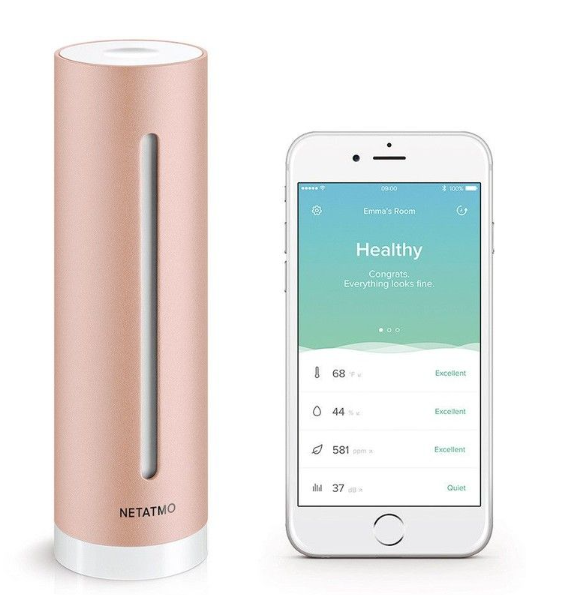
\includegraphics[width=0.4\textwidth]{figures/Netatmo.png}
    \caption{Netatmo Healthy Home Coach \cite{NetatmoDevice}}
    \label{fig:Netatmo}
\end{figure}
\\\\
In the privacy policy of Netatmo, the following personal data is stated that Netatmo store; unique ID of cookie, IP address, information about the equipment, information about user activity on webpage and app. They also state that they will collect and store measurements from the app to use in commercial campaigns. To be able to run and use the application, third party services are used by Netatmo. In addition, statistical data is collected to understand the users and their needs and add functionality accordingly.  
\\\\
The Netatmo Healthy Home Coach sends notifications to the users application when the device sense high temperature, \(CO_2\), humidity or noise and low temperature or humidity. These are default on, but can be turned off by the user. The values cannot be changed, but are stated by Netatmo in the app. The unit displays live readings to the user through the app, together with a graphical view of values over a longer period of time. When first installed, the devices needs at least 7 days to be able to calibrate and read the environment correctly. 


\section{Environment Setup}
\subsection{Air Quality Monitors}
It is desirable that the air quality monitors gives notifications when a certain threshold value is met. However, for Mill Sense it is not possible to set notifications. The MAC addresses for the air quality monitors can all be found in their corresponding apps. 

\begin{table}[!hbtp]
    \centering
    \begin{adjustbox}{width=1\textwidth}
    \begin{tabular}{| p{3cm} | p{5cm} | p{5cm} | p{3cm} |} 
        \hline
        \textbf{Air Quality Monitor} & \textbf{MAC Address} & \textbf{Threshold values for notifications} \\
        \hline
        Mill Sense Smart Climate sensor & B8:F0:09:B3:B3:78 & None \\
        \hline
        Nedis SmartLife Air Quality Monitor & 2C:F4:32:29:36:DC & \(CO_2\) > 1000 ppm \newline Humidity < 30\%  \newline Humidity < 50\% \newline Temperature < 15 \degree C \newline Temperature > 25 \degree C \newline VOC > 99.9 ppn\\
        \hline
        Netatmo Smart Air Quality Monitor & 70:EE:50:91:06:DE & \(CO_2\) > 1150 ppm \newline Noise > 62db \newline Humidity < 30\% \newline Humidity > 60\% \newline Temperature < 17 \degree C \newline Temperature > 26 \degree C \\\\
        \hline
    \end{tabular}
    \end{adjustbox}
    \caption{Air Quality Monitor Devices}
    \label{tab:AQMSurvey}
\end{table}
\subsection{Sniffer}
To be able to collect all Wi-Fi traffic within the environment, a network sniffer needs to be configured. It exists a wide variety of sniffers online for every communication protocol. However, the selected sniffer in this research is the TP-Link TL-WN722N. 
\\\\
\begin{figure} [!ht]
    \centering
    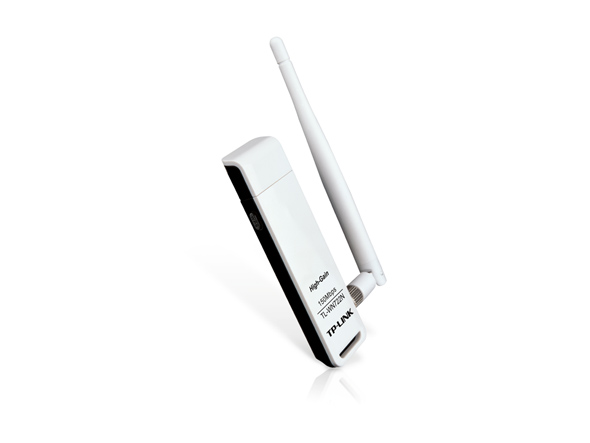
\includegraphics[width=0.3\textwidth]{figures/Sniffer.jpg}
    \caption{TP-Link TL-WN722N \cite{Sniffer}}
    \label{fig:Sniffer}
\end{figure}
\\\\
To set the device in monitoring mode, its first plugged into a computer, raspberry pie or similar and then the following commands are run. Wlan0 is the assigned wlan for the device when I plugged it into my environment, so it needs to be changed accordingly. 
\begin{verbatim}
    sudo ifconfig wlan0 down
    sudo iwconfig wlan0 mode monitor
    sudo ifconfig wlan0 up
    sudo iwconfig
\end{verbatim}
The sniffer is then ready to collect traffic from all devices communicating over Wi-Fi within its own signal range. 
\subsection{Tshark}
In order to store and process the traffic that the TP-link collects, a monitoring software was needed. Tshark is an open and free network packet analyzer and will be used to store packets. Tshark can be runned from the commandline and contains the possibilty of using capture filters based on a numerous parameters, such as addresses, duration or size. To be able to store the packets captured, tshark was runned with the option of writing its results to an output file rather than in the command line. The packets collected in the output file by tshark is possible to open and analyze in Wireshark. 

To be able to store packets from all the three air quality monitors, tshark was runned from three different terminals with the following three filters:
\begin{verbatim}
    For Mill Sense:
        
    For Nedis SmartLife:
        
    For Netatmo Healthy Home Coach:
        
\end{verbatim}

\subsection{Environment}
To be able to to collect data and store it from the devices, an operating system running on an hardware component to be able to connect the sniffer is needed. In this research, a Raspberry Pie installed with Kali Linux was chosen to be able to run the packet capturing continuously and have the needed software installed on the operating system. 

\section{Test Cases}
\subsection{Justification of test cases}
\subsection{Test Case 1: Cooking}
\subsection{Test Case 2: Showering}
\subsection{Test Case 3: Window open at night}